This chapter introduces the interprocedural analysis framework.
We have previously introduced the builtin framework and the
Tame IR. In the next chapter we will introduce the value analysis,
an interprocedural analysis that uses all these tools to build
a callgraph with annotated type information. In order to implement
this interprocedural analysis, we have developed the 
interprocedural analysis framework.

The interprocedural analysis framework builds on top of the
Tame IR and the \mcsaf intraprocedural analysis framework. It allows
the construction of interprocedural analyses by extending an
intraprocedural analysis built using the \mcsaf framework. This
framework works together with a callgraph object implementing the
correct \matlab look up semantics. An analysis can be run on an
existing callgraph object, or it can be used to build new callgraph
objects, discovering new functions as the analysis runs.

In the following sections we will introduce the interprocedural
analysis framework as an extension of the intraprocedural analysis
framework, and how it works in tandem with callgraph objects and the
lookup objects, as well as how the framework deals with recursion. To
help potential analysis writers, we have indicated the names of Java
classes that correspond to the contexts in bold.


\section{The Function Collection Object}

In order to represent callgraphs we use an object which we call
\textbf{FunctionCollection}. It is, as the name suggests, a collection
of nodes representing functions, indexed by so function
reference objects. Objects of type \textbf{FunctionReference} 
act as unique identifiers for functions. They store a function's
name, in which file it is contained if applicable, and what kind
of function it is (primary function, subfunction, nested function,
builtin function, constructor). For nested functions, it stores
in which function it is contained. Function reference objects
give enough information to load a function from a file.

Nodes in the function collection not only store the code of the
function and a function reference; they also provide information
about its environment. The node provides a \matlab function lookup
object which is able to completely resolve any function call
coming from the function. It includes information about the 
\matlab path environment and other functions contained in the same file.
The lookup information is provided given a function name, and optionally
an mclass name (to find overloaded versions); and will return
a function reference allowing the loading of functions.

The lookup information allows us to build a callgraph knowing only an
entry point and a path environment, and using semantics for finding
functions that correspond to the way \matlab finds functions at
runtime. This is bridging \rednote{the} gap between a dynamic language and 
static compilers, which usually require specifying what source
code files are required for compilation.

The simple function collection uses only the lookup information
contained in its nodes to built an approximation of a callgraph,
which is naturally incomplete. We have used it for the development
of the Tamer framework, as it provides a simple way to generate
a callgraph which excludes discovering overloaded calls and propagation
of function handles. We have implemented slightly different
versions of the function collection, which are described in the table below.

\begin{table}[htbp]
\begin{center}
\begin{tabularx}{\textwidth}{|l|X|} \hline
\textbf{\rednote{SimpleFunctionCollection}} &
A simple callgraph object built using \matlab lookup semantics excluding overloading.
Function Handles are loaded only in the functions where the handle is created.
Obviously this an incomplete callgraph, but may be used \rednote{by} software tools that
do not need a complete callgraph, and where the simplicity can be useful. \\ \hline
\textbf{IncrementalFunctionCollection} & callgraph that does the same lookup as 
the FunctionCollection, but does not actually load functions until they are requested.
This is used to build the callgraph \\ \hline
\textbf{CompleteFunctionCollection} &
callgraph that includes call sites for every function \rednote{node and} correctly
represents overloading can calling function handles. This is produced
by the Tamer using interprocedural analyses. This callgraph can be used to 
build further interprocedural analysis that are not extensions of the value
\rednote{analysis}. It can also be used as a starting point for static
backends.
\\ \hline
\end{tabularx}
\end{center}
\caption{The different kinds of Function Collection objects.}
\end{table}



\section{The Interprocedural Analysis Framework}
\label{sec:interprocedural}

The interprocedural analysis framework is an extension of the
intraprocedural flow analyses provided by the \mcsaf framework. It is
context-sensitive to aid code generation targeting static languages
like {\sc FORTRAN}. {\sc FORTRAN}'s polymorphism features are quite
limited; every generated variable needs to have one specific type. The
backend may thus require that every \matlab variable has a specific
known mclass at every program point. Functions may need to be
specialized for different kinds of arguments, which a
context-sensitive analysis provides at the analysis level.

An interprocedural analysis is a collection of interprocedural
analysis nodes, called \textbf{InterproceduralAnalysisNode}, which represent
a specific intraprocedural analysis for some function and some
context.
The context is usually a flow representation of the passed
arguments. Every such interprocedural analysis node produces a result
set using the contained intraprocedural analysis.
An InterproceduralAnalysisNode is generic in the intraprocedural analysis,
the context and the result - these have to be defined by an 
actual implementation of an interprocedural analysis.

Every interprocedural analysis has an associated FunctionCollection
object, which may initially contain only one function acting as the
entry point for the program (i.e. when building a callgraph using an
IncrementalFunctionCollection). The interprocedural analysis requires
a context (argument flow set) for the entry point to the program.

\subsubsection{Algorithm}

The analysis starts by creating an interprocedural analysis node
for the entry point function and the associated context, which
triggers the associated intraprocedural flow analysis. As the
intraprocedural flow analysis encounters calls to other functions, it
has to create context objects for those calls, and ask the
interprocedural analysis to analyze the called functions using the
given context. The call also gets added to the set of call edges
associated with the interprocedural analysis node.

As the interprocedural has to analyze newly encountered calls, the
associated functions are resolved, and loaded into the callgraph if
necessary. The result is a complete callgraph, and an interprocedural
analysis.

% for thesis: call objects, class diagrams, more about recursion

\subsection{Contexts}

In order to implement an interprocedural analysis, one has to define
a context object. These may be the flow information of the arguments
of a call; but it could be any information. The analysis itself
is context-sensitive, meaning that if there are multiple calls
to one function with different contexts, they are all represented
by different interprocedural analysis nodes. The interprocedural
analysis framework never merges contexts, which would have to be
done by the specific analysis if desired.

Interprocedural analysis nodes are cached. Thus if a function/context
pair is called a second time, the information will be readily available.

Note that in order to completely resolve calls, the flow information
and the contexts have to include mclass information for variables
and arguments. In order to resolve calls to function handles, the 
contexts have to store which arguments may refer to function handles
(and which functions they refer to).

Once the complete callgraph is built, further analyses
don't need to flow mclass information, because all possible calls
are resolved. But this information may still be useful
to obtain more accurate analysis result, by knowing
which information to flow into which calls for ambiguous
call sites (see \secref{sec:callsites}) - that is why the 
value analysis presented in \rednote{\chapref{chap:ValueAnalysis}}
allows extending the flow-sets, to allow flowing information
for different analyses together in one \rednote{analysis}, and get a 
more precise overall result.


\subsection{Call Strings}
\label{sec:callstrings}

When analyzing a function $f$ for a given context $c_f$, and
encountering a call to some other function $g$, the interprocedural
analysis framework suspends the analysis of $f$ in order to analyze
the encountered call. The flow analysis has to provide a context $c_g$
for the call to $g$, and an intraprocedural analysis will be created
that will analyze $g$ with $c_g$. 

\begin{figure}[htbp]
\begin{center}
\includegraphics[scale=.6]{Figures/callstring.eps}
\caption[A small program where $main$ calls $f$ calls $g$.]{
A small program where $main$ calls $f$ calls $g$. The call string
for $g(c_g)$ in this example may be $main(c_{main}) : f(c_f) : g(c_g)$.
}
\label{Fig:callstring}
\end{center}
\end{figure}


The set of currently suspended functions (in \figref{Fig:callstring}
$main$ and $f$), which are awaiting results of encountered calls that
need to be analyzed correspond to the callstack of these functions at
runtime, at least for non-recursive programs. We call the chain of
these functions, together with their contexts a \textbf{ CallString}. Every
function/context pair, i.e. the associated interprocedural analysis
node, has an associated call string, which corresponds to one possible
stack trace during runtime.  Note that interprocedural analysis nodes
are cached, and may be reused. Thus in the above example, if the main
function also calls $g$ with context $c_g$, the results of the
interprocedural analysis node created for the call encountered in
function $f$ will be reused.

\begin{figure}[htbp]
\begin{center}
\includegraphics[scale=.6]{Figures/branch.eps}
\caption[A small program showing two calls to a function]{
Here, $main$ also calls $g$, also with context $c_g$. Since the interprocedural analysis node
for $g(c_g)$ is reused, the call string will be reused as well.
}
\label{Fig:callstring}
\end{center}
\end{figure}


Since the interprocedural analysis node is reused, it will have the
same call string. So the call string is not an exact representation of
a call stack for every call, it is merely the exact representation of
one possible call stack that will reach a given function/context
pair. Note that for purposes of error reporting, the call string can
be presented to the user as a stack trace.

\subsection{Callsite}
\label{sec:callsites}

Any statement representing a call may actually represent multiple
possible calls. For example a call to a function $g$ may be
overloaded, so if arguments may have different possible mclasses,
different functions named $g$ may be called. Also, because it is up to
an actual analysis to define its notion of what a context is, it is
possible that an analysis may decide to produce multiple contexts for
one call to a function $f$. This would create specialized versions of
a function from a single call (this is actually possible in the value
analysis presented in \chapref{chap:ValueAnalysis}).  A third way in
which a statement may represent multiple possible calls is via
function handles. An TIRArrayGet statement may trigger a call if the
represented array is actually found to be a function handle (we call
the variable accessed in a TIRArrayGet statement an 'array'
simply because it is used in an array-indexing operation, but it 
could be any variable). If that function handle may refer to multiple
possible functions at runtime, then the function handle access may
refer to multiple possible calls.

\begin{figure}[htbp]
\begin{center}
\includegraphics[scale=.5]{Figures/callsites.eps}
\caption[Multiple possible callsites from one statement]{
This figure shows examples how it is possible for one single call site
to refer to multiple possible calls. This may \rednote{be} due to overloading,
creation of multiple contexts for a single call, or function handles.
}
\label{Fig:callstring}
\end{center}
\end{figure}

In order to be able to represent multiple possible call edges coming
out of a statement, we associate any statement that includes any calls
with a \textbf{Callsite} object. This callsite can store multiple
possible call edges as function/context pairs, which we call a
``call'' in the interprocedural analysis framework.  An
intraprocedural analysis, in order to request the result of a call,
has to request a callsite object for a calling statement. It may then
request arbitrary calls from that callsite object, which will all
get associated with the calling statement.

\subsection{Recursion}

The interprocedural analysis framework supports simple and mutual
recursion by performing a fixed point iteration within the first
recursive interprocedural analysis node. In order to identify
recursive and mutually recursive calls we use the call strings
introduced in \secref{sec:callstrings}. While we established that
there is no guarantee which stack trace the call string represents,
we know that it will always represent one possible stack trace.
Since the call stacks of all recursive and mutual recursive calls must
include the function, we merely need to check, for any call,
whether it already exists in its call string.

\begin{figure}[htbp]
\begin{center}
\includegraphics[scale=.6]{Figures/recursive.eps}
\caption[A recursive example]{
Example of a recursive program. The call in $s(c_s)$
to $f(c_f)$ triggers the fixed point iteration of $f(c_f)$. 
$f(c_f)$ is the first recursive interprocedural
analysis node.
}
\label{Fig:recursive}
\end{center}
\end{figure}


If it does, we have identified a recursive call, and must perform a
fixed point iteration. To do so, we label the intraprocedural analysis
node associated with the recursive call (i.e. the call to $f(c_f)$
in \figref{Fig:recursive})  as recursive. This will trigger the fixed point
iteration.  Because we need a result for the recursive call to
continue analyzing, an actual analysis implementation has to provide a
default value as a first approximation, which may be just bottom.
Once the intraprocedural contained in the interprocedural analysis
node associated with the recursive call is completed, the result is
stored as a new partial result. The analysis is then recomputed, using
this new partial result for the recursive call. When a new partial
result is the same as a previous partial result, we have completed the
fixed point iteration. Note that the computation resulting in the new
partial result uses the previous partial result for its recursive call
- but since they are the same, we have made a complete analysis using
the final result for the recursive call.

Note that the while the fixed point iteration is being computed, all
calls below the recursive call (i.e. the calls $g(c_g)$ and $s(c_s)$
in \figref{Fig:recursive}) always return partial results. Thus we
cannot cache the nodes and their results, and have to continuously
invalidate all the corresponding interprocedural analysis nodes.


\begin{figure}[htbp]
\begin{center}
\includegraphics[scale=.6]{Figures/chain.eps}
\caption[Example program showing an infinite chain of calls.]{
Example of a recursive program, showing how recursive calls
with different contexts can create infinite chains of calls on the left.
An interprocedural analysis implementation has to catch
such cases and create a finite number of contexts, as shown on 
the right, where the contexts $c_2$ and onward are replaced with $c'$.
In this case the interprocedural analysis framework will perform a
fixed point iteration on $f(c')$.}
\label{Fig:chain}
\end{center}
\end{figure}

Note that the analysis treats calls to the same function with 
different contexts as different functions. No fixed point iteration
is performed to resolve recursive calls with different contexts,
because they represent different underlying intraprocedural analyses.
Thus it is possible to create infinite call strings, as shown in 
\figref{Fig:chain}.
It is up to \rednote{the} actual analysis implementation to ensure this does not
happen. A simple strategy would be to ensure that there are only
a finite number of possible contexts for every function. Another strategy
is for the intraprocedural analysis to check the current call string
before requesting a call, to ensure that the function to be called
does not already exist in the call string. If it does, the intraprocedural
analysis should push up the context to a finite representation (shown 
in \figref{Fig:chain}).

\section{Summary}

We have presented an interprocedural analysis framework that we 
hope is flexible enough to allow different kinds of full-program analyses,
while powerful enough to deal with issues such as recursion and 
ambiguous call sites. This analysis framework is a key component
of our value analysis (presented in the next chapter), and the overall
callgraph construction of the Tamer.

